\section{Evaluation}\label{sec:eval}

In order to measure how interesting and interactive our \tube is, we developed our applications to be able to accept inputs from both traditional input devices (\ie mouse and keyboard) and our \tube. For instance, in the balloon popping game the user will be able shoot down the balloons by clicking them with the mouse. To match the balloons’ colors, the users will have to press corresponding keys on the keyboard.
After describing to our participants how \tube works, the participants tried out the applications that we have developed first with mouse and keyboard,and later with \tube as the input device.

% \marginpar{
% \begin{figure}
%   \begin{center}
%   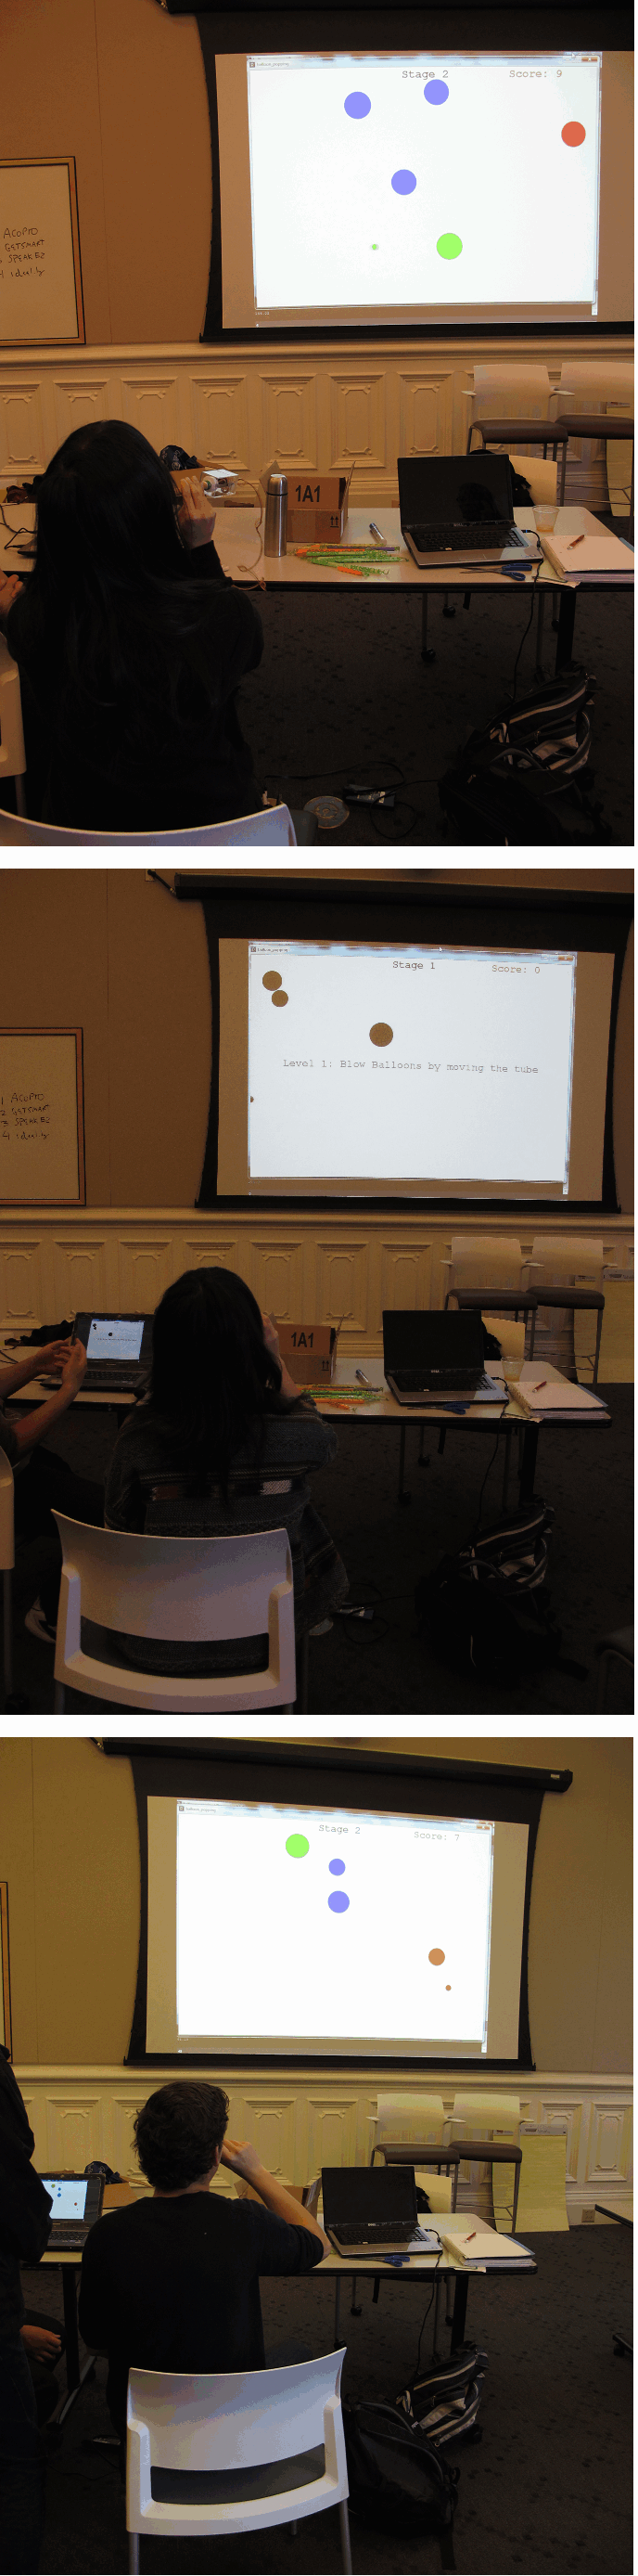
\includegraphics[width=0.7\marginparwidth]{./figs/eval.png}
%   \label{fig:eval}
%   \end{center}
% \end{figure}
% }

The first thing that our testers did when trying out the \tube was figuring how to control the small pointer on the screen. Since pointer is correspondingly moving on the screen, our testers adapted to the system naturally and in no time successfully played with \tube. Additionally, the bursting animation and sound that is generated whenever a balloon is popped gave the users a sense of accomplishment.

\begin{figure}
  \centering
  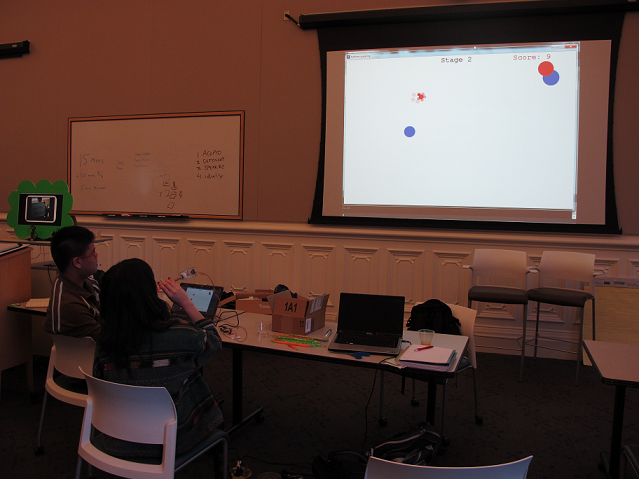
\includegraphics[width=\linewidth]{./figs/impl2.png}
  \caption{The participants trying out \tube during a project showcase on December 7th 2011 at UC Berkeley campus.}
  \label{fig:impl2}
\end{figure}

The challenging part is when the users have to match the color of the pointer with the color of the balloon by rotating the tube. It is not that obvious for our testers that they needed to rotate \tube in order to change the color of the pointer for this type of interaction is one of a kind. After observing that they could not pop the balloon without matching the colors, they started experimenting with orienting \tube in different positions and started blowing while rotating the tube. However, we may need to improve on our hardware design since some users lamented on the motion sensitivity of our \tube.
